\documentclass{article}

\usepackage[utf8]{inputenc}
\usepackage{graphicx}		% Graphics.
\usepackage{color}
\usepackage[english]{babel}
\usepackage{float}
\usepackage{subcaption}
\usepackage{xfrac}
\usepackage{matlab-prettifier}
\usepackage{amsmath}    
\usepackage{amssymb}
\usepackage{siunitx}
\usepackage{pdfpages}
\usepackage{hyperref}
\usepackage{longtable}
\usepackage{multicol}
\usepackage{enumitem}

% Create a separate table for the appendix.
\usepackage[toc,page]{appendix}

% Table of Content has fast links to sections.
\usepackage{hyperref}

% Remove dots in table of contents.
\usepackage[titles]{tocloft}
\renewcommand{\cftdot}{}

% Page style.
\usepackage[top=2cm, bottom=2cm, left = 2cm, right = 2cm]{geometry}
\setlength{\parindent}{0pt}	% Disable indents.

\begin{document}
	
	%----------------------------------------------------------------------------------------
	%	Title page.
	%----------------------------------------------------------------------------------------
	\begin{titlepage}
		\center
		\newcommand{\HRule}{\rule{\linewidth}{0.5mm}}
			\textsc{\Huge Battle of the Neighbourhoods}\\[1.5cm]
			\textsc{\LARGE Applied Data Capstone - Coursera}\\[0.3cm]
			\textsc{\large Diego Talavera}\\[0.5cm]
		
			\vfill\vfill\vfill % Position the date 3/4 down the remaining page.
			
			{\large\today} % Date, change the \today to a set date if you want to be precise.
	\end{titlepage}
	
	
	%----------------------------------------------------------------------------------------
	%	TABLE OF CONTENT.
	%----------------------------------------------------------------------------------------
	\newpage				% Start at new page.
	\pagenumbering{arabic}	% Page numbering reset & style.
	\renewcommand{\contentsname}{Table of Contents}
	\tableofcontents		% Add table of content.
	
	%----------------------------------------------------------------------------------------
	% 	INTRODUCTION
	%----------------------------------------------------------------------------------------
	
	\newpage
	\section{Introduction}
	\subsection{Problem Description}
		Imagine that you need to buy several very different items. From groceries, to furniture, so some electronics, etc. And you would like to buy all of these items on a single trip. You are willing to travel up to \SI{50}{\kilo\meter} in any direction but all the stores you need, should be close to each other. Here are some other factors that will be taken into account to choose the best neighbourhood: 
		\begin{itemize}
			\item The average rating of the stores in a given cluster
			\item The distance from your starting point
			\item The average distance between the stores in a given cluster
			\item The opening hours of the venues on different days
		\end{itemize}
		
		With this all this information, you could then choose the best neighbourhood and day of the week to do your shopping. 
	
	\subsection{Description and use of data}
		In this section, the data will be described, as well as some assumptions needed to simplify the analysis. The methods to be used are also presented here. 
		
		\subsubsection{Data requirements}
		\begin{itemize}
			\item \textbf{Shopping List:} First, a simple dataframe of items to be bought that includes the category of said item, this will be used to determine what kind of stores to look for 
			\item \textbf{Location Data:} A starting point will be chosen within the city of Stockholm, Sweden. The location of the other venues will also be used to calculate the distance to the starting point
			\item \textbf{Venues information:} 3 main pieces of information will be needed in this case: The category of the venue, the opening times and the rating of the venue. 			
		\end{itemize}
		\subsubsection{Data usage and assumptions}
			In order to make the data analysis less complicated, the assumptions and considerations are as follows:
			\begin{itemize}
				\item Instead of looking at the prices for each item in each store, the rating of the store will be used paired with the distance to the starting point in order to take a decision. This can still be relevant since most people give good ratings to stores that have a good price-to-quality ratio.
				\item Only straight-line distance will be used (instead of, say, the driving distance, which will vary since not every single street in a city is straight, duh!).
				\item An overall "Likelihood score" will be developed to choose the best store cluster. For example, the distance from the starting to each cluster will have a \textit{negative} impact on said score, but the mean customer rating will have a \textit{positive} impact. The specific ratio of how each parameter affect this score will be determined later in the study.
			\end{itemize} 	
		\newpage
		\subsubsection{Methods}
			First, Pandas will be used to create our starting dataframe with the shopping list and the categories for each item. Data from the venues around our starting point, will be obtained with the Foursquare API. This data will then also be put into a dataframe for further exploratory analysis. A clustering algorithm can then be used to divide the venues into clusters, hopefully obtaining something similar to the image below:
			
			\begin{figure}[H]
				\centering
				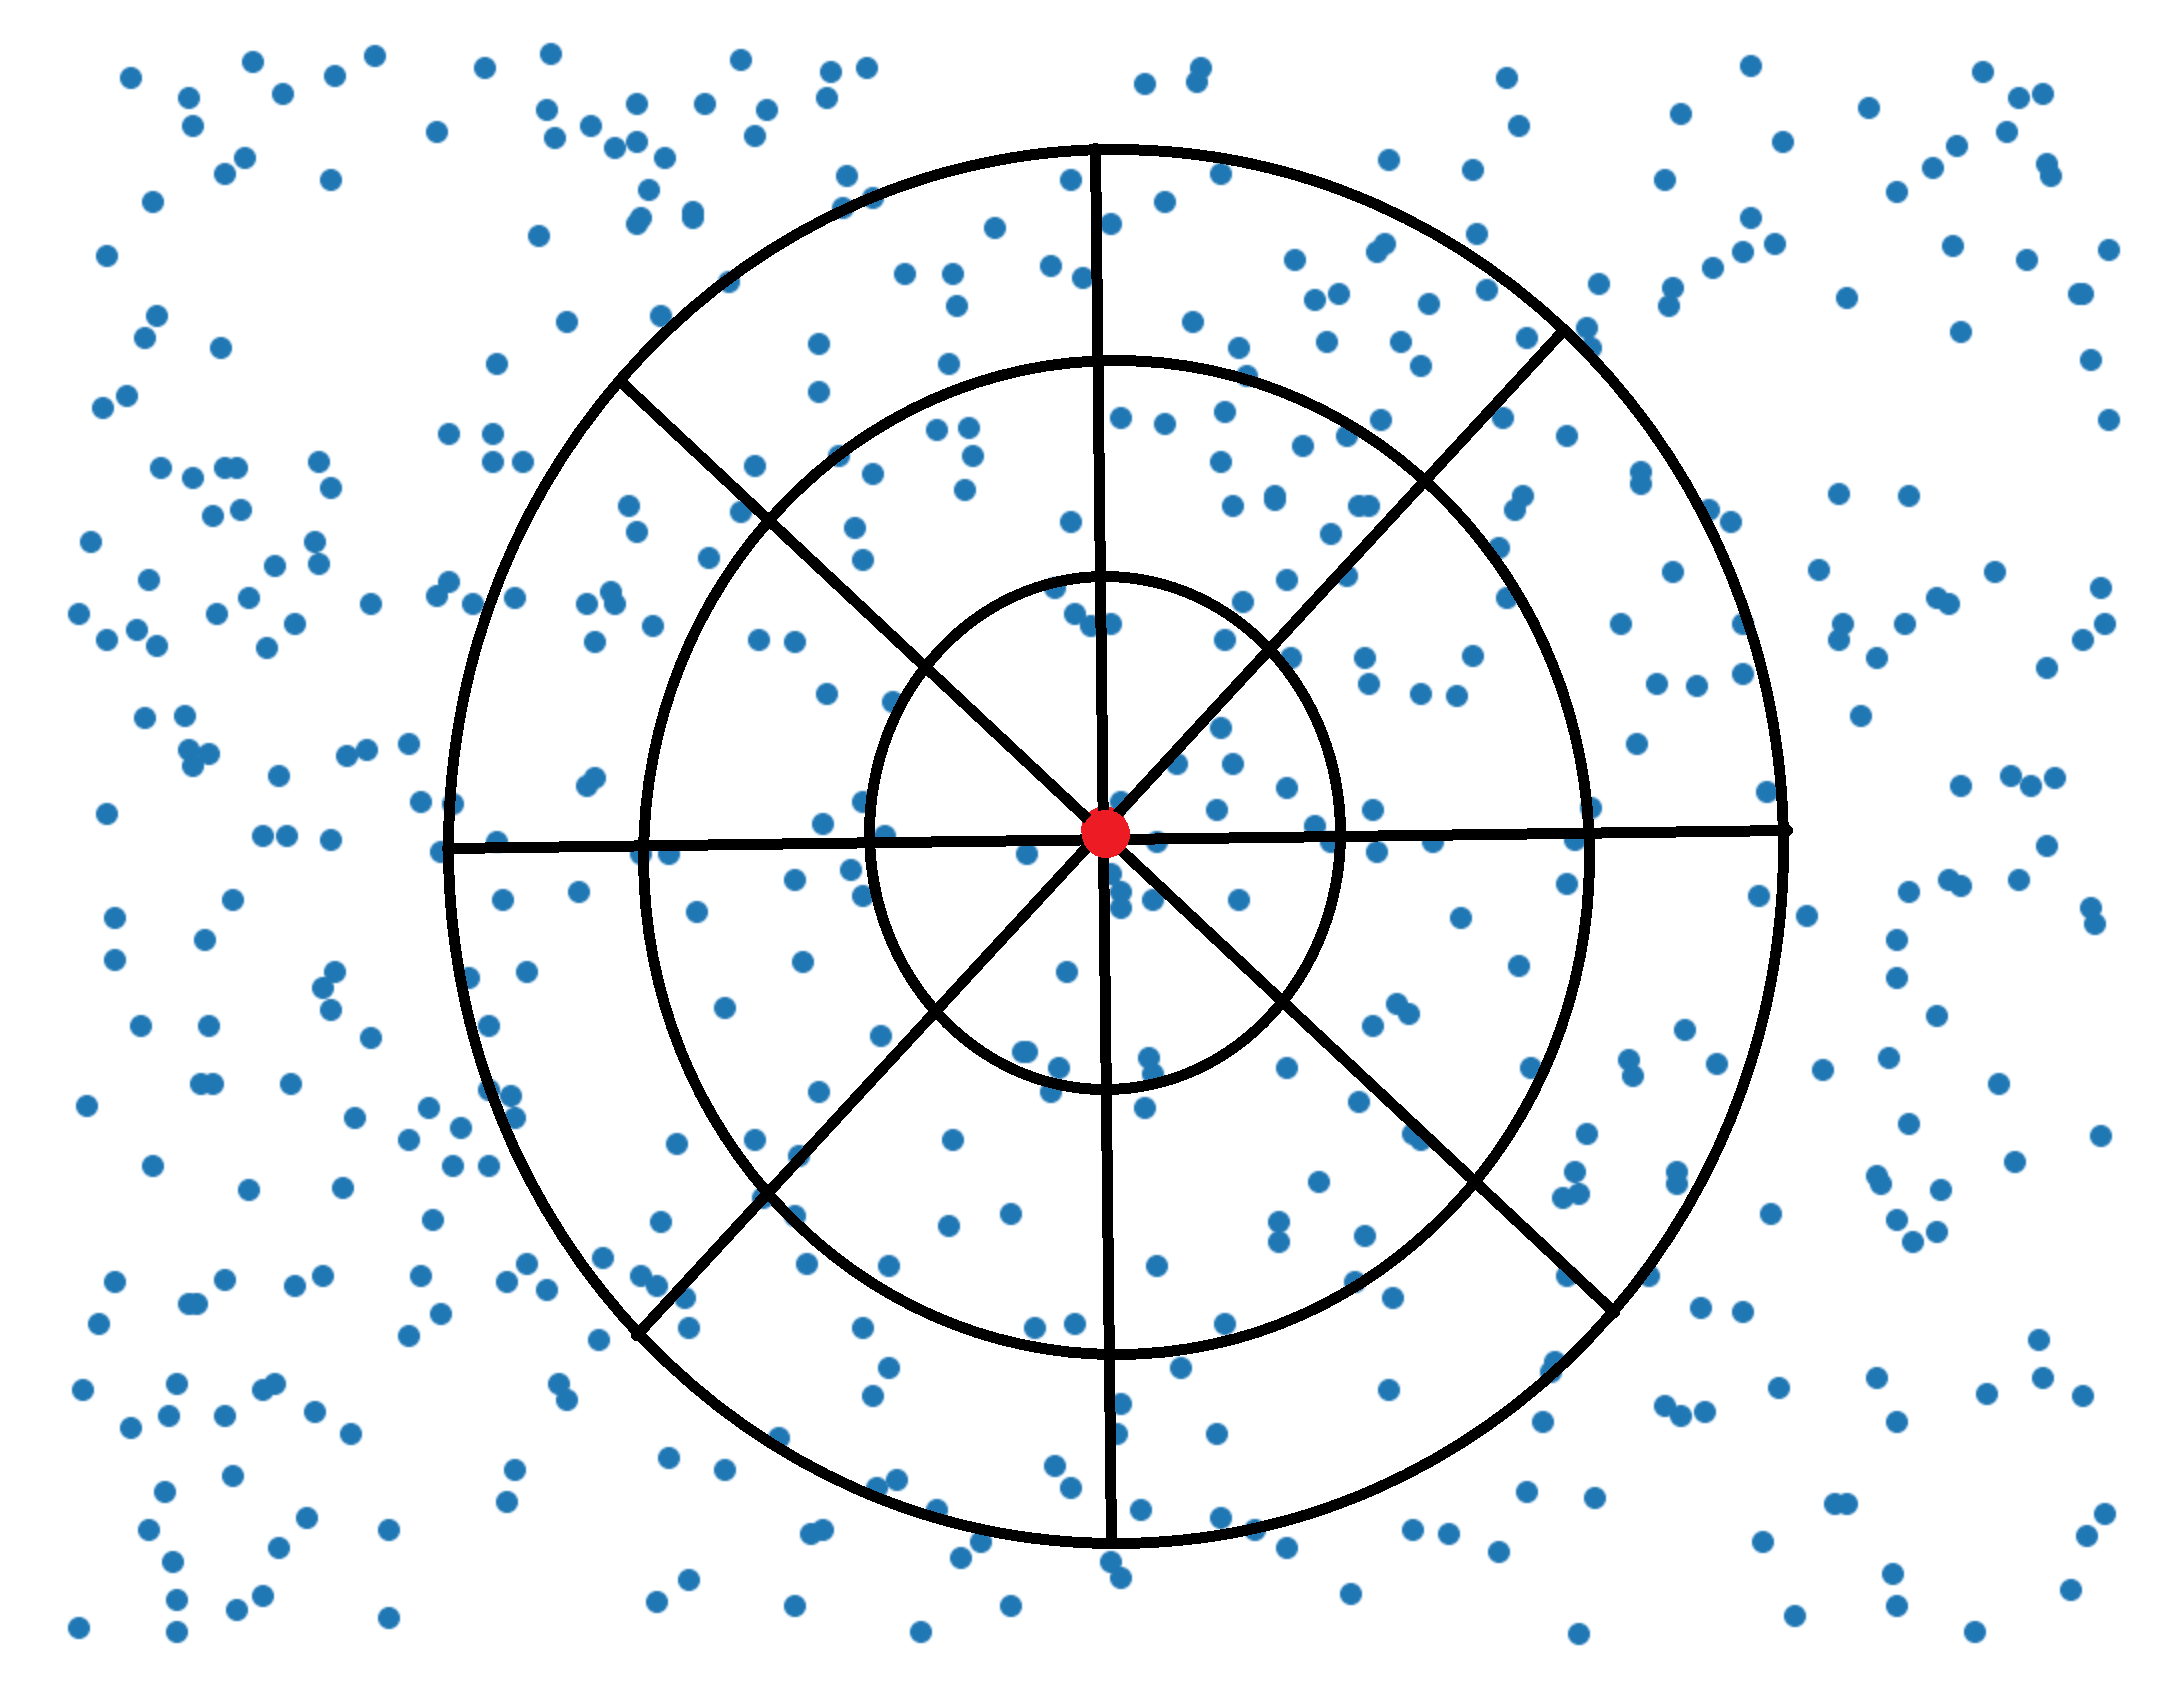
\includegraphics[width=0.5\textwidth]{img/Expected.png}
				\caption{Expected clustering for the venues. Note that this is just an example and it has a scatter plot with randomized points in the background. Red point represents the starting point}
			\end{figure}
		
		
			This will likely be achieved by using a clustering algorithm "twice": once on the raw data, and then one more time to subdivide each cluster into sub cluster. This will be especially handy, since the expected main clusters will be expected to be rings around the starting point. So, maybe the farthest ring would have the best score, but the stores are diametrically opposed, which would result in a very inefficient trip since it will double the already long distance of your shopping trip.
			\newline
			\newline			
			Afterwards, the "Likelihood score" of each individual cluster will be calculated, and used to choose the better cluster to do the shopping.
	
	
	
	
	
	
	
	
	
\end{document}
